\documentclass[12pt]{report}
\usepackage[utf8]{inputenc}
\usepackage{titlesec}
\usepackage[slovene]{babel}
\usepackage{acro}
\usepackage{amsmath}
\usepackage{textgreek}
\usepackage{graphicx}
\usepackage{float}
\usepackage[twoside]{fancyhdr}
\usepackage{etoolbox}
\usepackage{nomencl}
\usepackage{longtable}
\usepackage{tocloft}
%\patchcmd{\chapter}{\thispagestyle{plain}}{\thispagestyle{fancy}}{}{}
\makenomenclature
\RequirePackage[backend=biber,style=numeric]{biblatex}

\addbibresource{sources.bib}
\setcounter{tocdepth}{3}
\setcounter{secnumdepth}{3}

%Višina celice v tabeli
\renewcommand{\arraystretch}{1.1}

%Preimenovanje poglavij
\titleformat{\chapter}[display]
{\bfseries}{}{0pt}{\Huge\thechapter\quad}

% =========================== Okrajšave ==============================

\DeclareAcronym{PZF}{
  short=PZF,
  long=pasovno zavrnitveni filter,
}
\DeclareAcronym{MM}{
  short=MM,
  long= Metamateriali,
}
\DeclareAcronym{EVP}{
  short=EVP,
  long= problem lastnih vrednosti,
}

\DeclareAcronym{OC}{
  short=OC,
  long= osnovna celica,
}

\DeclareAcronym{FFF}{
  short=FFF,
  long= Fused Filament Fabrication,
}

% =========================== Simboli ==============================
\nomenclature[A]{$\mathbf{M}$}{globalna masna matrika}
\nomenclature[A]{$\mathbf{C}$}{globalna dušilna matrika}
\nomenclature[A]{$\mathbf{K}$}{globalna togostna matrika}
\nomenclature[A]{$\mathbf{q}$}{vektor generaliziranih vozliščnih pomikov}
\nomenclature[A]{$\mathbf{f}$}{vektor generaliziranih vozliščnih sil}
\nomenclature[G]{$\omega$}{krožna kotna frekvenca}
\nomenclature[A]{$t$}{čas}
\nomenclature[A]{$i$}{imaginarna komponenta}
\nomenclature[G]{$\rho$}{gostota}
\nomenclature[A]{$A$}{površina prereza}
\nomenclature[A]{$l$}{dolžina končnega elementa}
\nomenclature[A]{$E$}{elastični modul}
\nomenclature[A]{$I$}{vztrajnostni moment prereza}
\nomenclature[A]{$\mathbf{r}$}{krajevni vektor}
\nomenclature[A]{$\mathbf{k}$}{valovni vektor}
\nomenclature[A]{$L$}{dolžina bazne celice}
\nomenclature[A]{$n$}{število baznih celic med točkama}
\nomenclature[G]{$\mathbf{\mu}$}{vektor širjenja valovanja}
\nomenclature[A]{$\mathbf{t}$}{bazni translacijski vektor recipročne bazne celice}
\nomenclature[A]{$\mathbf{D}(\omega)$}{dinamska matrika sistema}
\nomenclature[G]{$\mathbf{\Lambda}_R$}{desna reducirna matrika}
\nomenclature[G]{$\mathbf{\Lambda}_L$}{leva reducirna matrika}
\nomenclature[A]{$\mathbf{I}$}{identična matrika}
\nomenclature[A]{$\mathbf{d}$}{bazni translacijski vektor bazne celice}

\renewcommand{\nomname}{Seznam simbolov}
\renewcommand\nomgroup[1]{%
  \item[\bfseries
  \ifstrequal{#1}{A}{Arabski simboli}{%
  \ifstrequal{#1}{G}{Grški simboli}{}}%
]}


\begin{document}
% ---- Oblikovanje strani
\pagenumbering{roman}

\renewcommand{\chaptermark}[1]{\markboth{#1}{}}
\fancyhf{}
\fancyhead[RO,RE]{\leftmark}
\fancyfoot[CO, CE]{\thepage}

% ---- Konec oblikavanja strani

\begin{titlepage}
    \begin{center}
        \textbf{UNIVERZA V LJUBLJANI}
        \\Fakulteta za strojništvo

        \vspace{5cm}
        \textbf{\Huge{3D natisnjeni metamateriali za aplikacijo v dinamiki}}

        \vspace{1cm}
        Seminarska naloga pri predmetu Dinamika togih teles

        \vspace{2cm}
        \textbf{\Large{Marko Zupan}}

        \vspace{4cm}
        Mentor: asist. Tilen Košir
        \\Somentor: prof. dr. Janko Slavič, univ. dipl. inž.

        \vspace{1.5cm}
        Ljubljana, december 2022


    \end{center}
    
\end{titlepage}

%Vsebinsko kazalo
\pagestyle{plain}
\vspace*{0mm}
\noindent\Large\textbf{Kazalo}\normalsize
\vskip\medskipamount
\leaders\vrule width \textwidth\vskip0.4pt
\vskip\bigskipamount
\makeatletter
\renewcommand{\tableofcontents}{\@starttoc{toc}}
\makeatother
\tableofcontents
\newpage



%Kazalo slik
\vspace*{0mm}
\noindent\Large\textbf{Kazalo slik}\normalsize
\vskip\medskipamount
\leaders\vrule width \textwidth\vskip0.4pt
\vskip\bigskipamount
\addcontentsline{toc}{section}{Kazalo slik}
\makeatletter
\renewcommand{\listoffigures}{\@starttoc{lof}}
\makeatother
\renewcommand\cftfigpresnum{Slika~}
\renewcommand\cftfigaftersnum{:}
\newlength{\mylen} % a "scratch" length
\settowidth{\mylen}{\bfseries\cftfigpresnum\cftfigaftersnum} % extra space
\addtolength{\cftfignumwidth}{\mylen} % add the extra space
\setlength{\cftfigindent}{0pt}
\listoffigures

\newpage
%Kazalo tabel
\vspace*{0mm}
\noindent\Large\textbf{Kazalo preglednic}\normalsize
\vskip\medskipamount
\leaders\vrule width \textwidth\vskip0.4pt
\vskip\bigskipamount
\addcontentsline{toc}{section}{Kazalo preglednic}
% Seznam tabel
\makeatletter
\renewcommand{\listoftables}{\@starttoc{lot}}
\makeatother

\renewcommand\cfttabpresnum{Preglednica~}
\renewcommand\cfttabaftersnum{:}
\settowidth{\mylen}{\bfseries\cfttabpresnum\cfttabaftersnum} % extra space
\addtolength{\cfttabnumwidth}{\mylen} % add the extra space
\setlength{\cfttabindent}{0pt}

\listoftables

\newpage
\vspace*{0mm}
\noindent\Large\textbf{Seznam uporabljenih simbolov}\normalsize
\vskip\medskipamount
\leaders\vrule width \textwidth\vskip0.4pt
\vskip\bigskipamount

\addcontentsline{toc}{section}{Seznam uporabljenih simbolov}
\begin{longtable}[l]{@{}p{.15\textwidth}@{}p{.15\textwidth}@{}p{.7\textwidth}@{}}
\hline
Oznaka & Enota & Pomen\\
\hline
\endfirsthead
\hline
\endhead
&&\\
$\mathbf{C}$ & N s m$^{-1}$ & globalna dušilna matrika\\
$\mathbf{d}$ & m & bazni translacijski vektor osnovne celice \\
$\mathbf{D}(\omega)$ & N & dinamska matrika sistema \\
$\mathbf{f}$ & N & vektor generaliziranih vozliščnih sil \\
$\mathbf{I}$ & / & identična matrika\\
$\mathbf{K}$ & N m$^{-1}$ & globalna togostna matrika \\
$\mathbf{k}$ & m$^{-1}$ & valovni vektor \\
$\mathbf{M}$ & kg & globalna masna matrika\\
$\mathbf{q}$ & m & vektor generaliziranih vozliščnih pomikov \\
$\mathbf{r}$ & m & krajevni vektor \\
$\mathbf{t}$ & m & bazni translacijski vektor recipročne osnovne celice \\
$A$ & m$^2$ & površina prereza \\
$E$ & GPa & elastični modul \\
$I$ & m$^4$ & vztrajnostni moment prereza \\
$i$ & / & imaginarna komponenta \\
$L$ & m & dolžina osnovne celice \\
$l$ & m & dolžina končnega elementa \\
$n$ & / & število baznih celice med točkama \\
$t$ & s & čas \\
&&\\
$\mathbf{\Lambda}_L$ & / & leva reducirna matrika\\
$\mathbf{\Lambda}_R$ & / & desna reducirna matrika\\
$\mu$ & m$^{-1}$ & vektor širjenja valovanja\\
$\omega$ & rad s$^{-1}$ & krožna kotna frekvenca\\
$\rho$ & kg m$^{-3}$ & gostota\\
\end{longtable}

\newpage
\thispagestyle{plain}
\vspace*{0mm}
\noindent\Large\textbf{Seznam uporabljenih okrajšav}\normalsize
\vskip\medskipamount
\leaders\vrule width \textwidth\vskip0.4pt
\vskip\bigskipamount

\addcontentsline{toc}{section}{Seznam uporabljenih okrajšav}

\begin{longtable}[l]{@{}p{.2\textwidth}@{}p{.8\textwidth}@{}}
\hline
Okrajšava & Pomen\\
\hline
\endfirsthead
\hline
\endhead
&\\
EVP & problem lastnih vrednosti (ang. \emph{Eigen Value Problem})\\
FFF & Fused Filament Fabrication \\
MM & metamaterial\\
OC & osnovna celica\\
PZF & pasovno zavrnitveni filter\\
\end{longtable}

\pagestyle{fancy}

\chapter{Uvod}
\pagenumbering{arabic}
\section{Cilji naloge}

Cilj naloge je izdelati numerični model in delujoč metamaterial, ki bo dušil vibracije
v željenem frekvenčnem območju. Specifično smo v okrivu naloge iskali območje dušenja
znotraj intervala 0 - 1000 Hz. Proces je bil razdeljen na 3 glavne podsklope.
\\
\\
V poglavju 2 so predstavljene teoretične osnove, ki jih potrebujemo za fizikalno razumevanje
problem in razvoj matematičnega modela, ki je osnova končnega numeričnega modela. Opisana je 
teorija nihanja sistemov z večimi prostostnimi stopnjami in teorija periodičnih struktur.
V poglavju 3 je predstavljen proces konstrukcije bazne celice in izdelave numeričnega modela. 
Opisani so osnovni koraki izdelave numeričnega modela ter predstavljeni koraki konstrukcije
osnovne celice.
V poglavju 4 je predstavljen eksperimentalni del s komentarji dobljenih rezultatov in primerjavo
z numeričnem modelom. Opisane so meritve in proces 3D tiska metamateriala.

\chapter{Teoretično ozadje}

\section{Uvod v metamateriale}
\ac{MM} so na makro nivoju posebno načrtovane strukture, ki imajo zaradi posebne geometrije izboljšane
mehanske lastnosti, kakršnih ne najdemo v naravi. \ac{MM} se uprabljajo na različnih področjih,
med njimi tudi v dinamiki. Na tem področju nas zanimajo \ac{MM}, ki so sposobni tvoriti \ac{PZF}. \ac{PZF} 
predstavlja frekvenčno področje, v katerem \ac{MM} teoretično ne dopušča prostega širjenja valovanja.
Znotraj takih področij lahko zato pričakujemo močno slabljenje vibracij.
\\
\\
\ac{PZF} lahko kreiramo prek dveh različnih mehanizmov. Prvi uporablja fizikalni princip Braggovega sipanja
 (ang. Bragg Scattering). Značilnost tovrstnega principa je periodična struktura \ac{MM} iz osnovnih gradnikov,
 ki vsebujejo visoke impedančne spremembe. To povzroča sipanje valovnih dolžin, ki so primerljive karakterističi dolžini 
 osnovnega gradnika. Pri Braggovem sipanju prihaja do destruktivne interference prihajajočega in odbitega vala, kar povzroči
 delno ali popolno izničenje valov. Ta princip je primeren le za tvorbo \ac{PZF} pri višjih frekvencah, kar ne ustreza
 ciljem te naloge.
 \\
 \\
 Drugi mehanizem deluje na principu lokalnih resonanc \ac{MM}. V okviru tega mehanizma na strukturo periodično namestimo
 lokalne resonatorje. Resonančni \ac{PZF} v tem primeru ni odvisen od periodičnosti, temveč geometrijskih lastnosti resonatorja. 
 Pogoja za nastanek \ac{PZF} sta majhna medsebojna oddaljenost resonatorjem (nekaj velikostnih razredov nižje od valovnih dolžin frekvenc,
 ki bi jih radi dušili) in ne-ničelna inducirana rezultantna sila na osnovno strukturo. Prednost tovrstnega pristopa je zmožnost kreiranja
 \ac{PZF} tudi pri nižjih frekvencah, slabosta pa, da lahko izven tega področja tudi močno poslabšamo slabljenje vibracij. \cite{kosir}
 \\
V okrviru te naloge se bomo osredotičli na konstruiranje 1D \ac{MM} preko mehanizma lokalnih resonatorjev.

\section{Osnove lastnih nihanj sistemov z več prostostnimi stopnjami}
V okviru tega poglavja predpostavimo, da že poznamo enačbe opazovanega sistema z več prostostnimi stopnjami, kot je 
prikazano na enačbi (2.1), kjer upoštevamo viskozni model dušenja, čeprav bomo tega v nadaljenaju zanemarili.

\begin{equation}
  \mathbf{M} \mathbf{\ddot{q}}(t) + \mathbf{C} \mathbf{\dot{q}}(t) + \mathbf{K} \mathbf{q}(t) = \mathbf{f}(t)
\end{equation}
\\
Kjer \textbf{M} predstavlja masno matriko sistema, \textbf{C} dušilno matriko sistema, \textbf{K} togostno matriko sistema, \textbf{x}(t) in \textbf{f}(t)
pa sta vektorja generaliziranih pomikov in vzbujevalnih sil.
V nadaljevanju predpostavimo harmonski odziv, zato lahko vektor pomikov in vektor generaliziranih vzbujevalnih sil zapišemo po enačbi (2.2).

\begin{equation}
  \mathbf{q}(t)=\mathbf{q} \sin{(\omega t)} =\mathbf{q}e^{i\omega t} \\
  \mathbf{f}(t)=\mathbf{f} \sin{(\omega t)} =\mathbf{f}e^{i\omega t}
\end{equation}
\\
Kjer \textbf{q} predstavlja vektor amplitud generaliziranih pomikov, \textbf{f} pa vektor generaliziranih vzbujevalnih sil. Če enačbo (2.1) preuredimo s pomočjo enačbe (2.2) dobimo sledečo enačbo
(2.3).

\begin{equation}
  (-\omega^2 \mathbf{M} + \mathbf{K}) \mathbf{q} = \mathbf{f}
\end{equation}
\\
V okviru naše naloge nas zanimajo lastne frekvence. Te dobimo iz netrivialne rešitve enačbe (2.3), ki jo dobimo z rešitvijo enačbe (2.4).
Problem prevedemo na problem lastnih vrednosti, ki je numerično stabilnejši.

\begin{equation}
  \textrm{det} (-\omega^2 \mathbf{M} + \mathbf{K})=0  
\end{equation}

\section{Metoda končnih elementov}
Metoda končnih elementov je aproksimativna metoda za reševanje matematičnih modelov in je najbolj razširjena med vsemi aproksimativnimi metodami.
Za naš primer bi lahko uporabili tudi metodo končnih elementov ali metodo robnih elementov, vendar je zaradi narave problema metoda končnih elementov najprimernejša.
S pomočjo te metode bomo pridobili globalno masno in togostno matriko \textbf{M} in \textbf{K}. 
\\
Osnovnih togostnih (2.5) in masnih (2.6) matrik za nosilec s štirimi prostostnimi stopnjami tu ne bomo izpeljevali, vendar jih pridobimo iz vira \cite{ville}.

\begin{equation}
  \mathbf{M} = \frac{\rho A l}{420} 
  \begin{bmatrix}
    156 & 22l & 54 & -13l \\
    22l & 4l^2 & 13l & -3l^2 \\
    54 & 13l & 156 & -22l \\
    -13l & -3l^2 & -22l & 4l^2
  \end{bmatrix}
\end{equation}
\begin{equation}
  \mathbf{K} = \frac{EI}{l^3} 
  \begin{bmatrix}
    12 & 6l & -12 & 6l \\
    6l & 4l^2 & -6l & 2l^2 \\
    -12 & -6l & 12 & -6l \\
    6l & 2l^2 & -6l & 4l^2
  \end{bmatrix}
\end{equation}
\\
Kjer je $\rho$ gostota, A površina preseka, l dolžina elementa, E elastični modul materiala in I vztrajnostni moment prereza.

\section{Osnove neskončnih periodičnih struktur}
Metamateriali so zaradi njihove narave navadno periodične stukture, kjer se v intervalih ponavlja osnovna celica.
Obravnavo problema si lahko olajšamo, kadar imamo neskončno periodično strukturo, saj takrat s pomočjo Bloch-Floquetovega teorema lahko 
preučujemo le odziv ene osnovne celice in tega generaliziramo na celotno strukturo.

\subsection{Bloch-Floquetov teorem}
V okviru te točke bomo predstavili osnove Bloch-Floquetovega teorema, ki ga potrebujemo za obravnavo našega problema.
Teorem nam pove, na kakšen način smemo obravnavati osnovno celico, da s tem popišemo celotno neskončno periodično strukturo \ac{MM}. \\
Omejimo se na 1D translatorno periodično strukturo z dolžino osnovne celice L. Za takšno periodično strukturo definiramo referenčni vektor $\mathbf{r}_U$, 
ki definira referenčno točko U, in referečno vektor $\mathbf{r}_P$, ki definira poljubno točko P na periodični strukturi. \cite{vanbelle, kosir}
\\Povezava je prikazana na sliki 2.1 in v enačbi (2.7).

\begin{figure}[H]
  \centering
  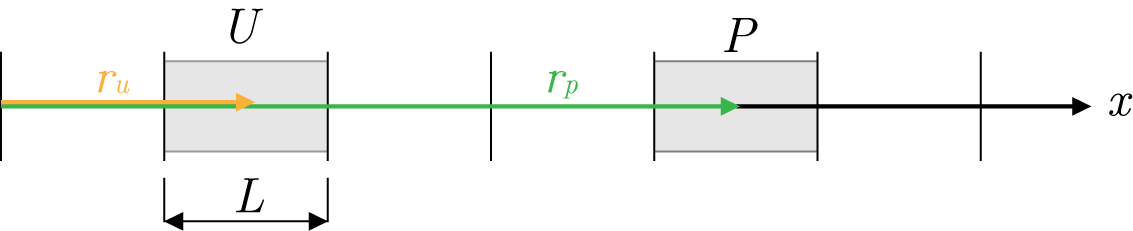
\includegraphics{Images/bloch.png}
  \caption{Prikaz 1D periodične strukture in njene bazne celice}
\end{figure}
\begin{equation}
  \mathbf{r}_P = \mathbf{r}_U + nL
\end{equation}
Kjer L ponazarja dolžino bazne celice, n pa celo število, ki pove število bazih celic med točkama U in P. Ponovno predpostavimo harmonsko
nihanje in tako lahko enačbo preuredimo kot:
\begin{equation}
  \mathbf{q}(r, k, t)  = \widetilde{\mathbf{q}}(r, k)e^{ik r}e^{i\omega t}
\end{equation}
Kjer r predstavlja pozicijo na x poltraku, $\omega$ frekvenco valovanja, k valovno število v smeri širjenja valovanja i pa kompleksno število. Na podlagi odziva referenčne celice
v točki U lahko napovemo odziv v katerikoli točki. Prav tako definiramo še kompleksno število širjenja valovanja $\mu$, ki nam fizikalno predstavlja fazni zamik. Preoblikovano enačbo zapišemo
kot:
\begin{equation}
  \mathbf{q}(r_P, \mu, t)  = \mathbf{q_{ref}}(r_U, \mu,t)e^{i\mu n}
\end{equation} 
Preko odziva osnovne celice lahko torej ob predpostavki neskončne periodične strukture modeliramo in napovemo odziv po celotni
periodični strukturi.

\subsection{Izračun disperzijskih krivulj}
Osnova analize širjenja valovanja znotraj osnovne strukture \ac{MM} je izračun disperzijskih krivulj. S konstrukcijo reprezentativne
osnovne celice in uporabo Bloch-Floquetovega teorema pridobimo disperzijski \ac{EVP} za frekvenco $\omega$ in valovni vektor $\mu$. \cite{vanbelle}

\subsubsection{Brillouinove cone}
Da lahko iz ravnin preidemo v krivulje, izkoriščamo periodičnost in simetrijo. Ker analiziramo periodično strukturo lahko določimo periodo 2$\pi$ za Re($\mu$) v recipročnem prostoru.
Problem razdelimo v tako imenovane Brillouinove cone. \cite{vanbelle}
\\Brillouinova cona je definirana kot Wigner-Seitzova celica v recipročnem prostoru. Najmanjši prostor, ki ga definira Wigner-Seitzova celica imenujemo prva Brillouinova cona.\cite{abhipod} Prva Brillouinova cona
je najmanjši osnovni gradnik, na podlagi katerega lahko popišemo celotno periodično strukturo. Če upoštevamo še simetrijo osnovne celice je možno slednjo cono še dodatno reducirati na nereducirno Brillouinovo cono. Ta predstavlja najmanjši prostor,
ki ga je potrebno obrvnavati, da popišemo celotni odziv osnovne celice in posledično celotnega \ac{MM}. \cite{kosir}
\\
\\
V sklopu te naloge bomo obravnavali 1D strukturo, zato se problem močno poenostavi. V ravninskem primeru bazni vektor celice \textbf{d} in bazni vektor recipročne celice \textbf{t} sovpadata s koordinatno osjo x. Poznamo tudi periodičnost, ki je enaka 2$\pi$. 
Celico transformiramo na dimenzije $[-\pi, \pi]$ s koordinatnim sistemom $\mu$, kot je prikazano na sliki (2.3).

\begin{figure}[H]
  \centering
  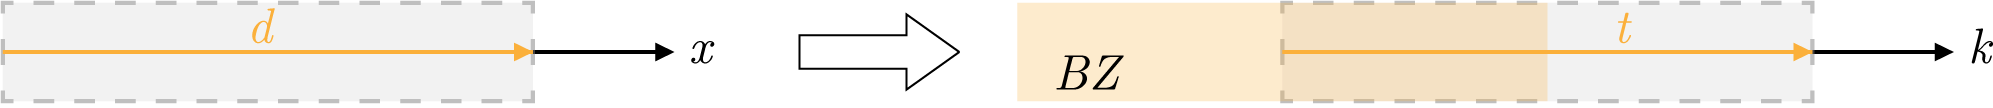
\includegraphics[scale=0.8]{Images/osnovna_celica.png}
  \caption{Bazne celice, njena recipročna celica v prostoru in Brillouinova cona (BZ)}
\end{figure}
\begin{figure}[H]
  \centering
  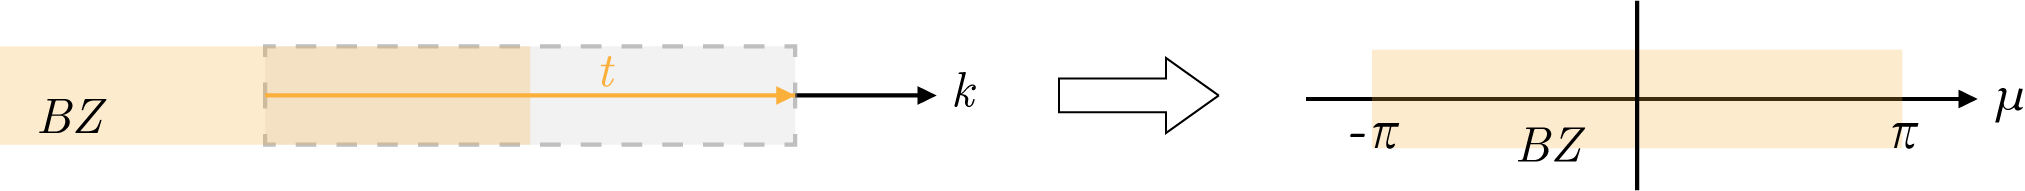
\includegraphics[scale=0.8]{Images/transformacija.png}
  \caption{Transformacija Brillouinove cone iz valovnega (k) v valovni ($\mu$) prostor}
\end{figure}

\subsubsection{Modeliranje osnovne celice}
V poglavju 2.2 smo izpeljali vodilno enačbo problema (2.3), kjer smo dobili dinamsko matriko:
\begin{equation}
  \mathbf{\hat{D}}(\omega)= -{\omega}^2 \mathbf{M}+K
\end{equation}
Sledeča dinamska matrika zaenkrat še ne vključuje nobenih robnih pogojev. V nadaljevanju bomo z uporabo Blochovega teorema za našo
dinamsko matriko določili periodične robne pogoje. Končna celica bo v numeričnem modelu imela več kot le dve vozlišči, zato v naslednjem koraku vektor pomikov $\mathbf{\hat{x}}$
razdelimo na pomike v levem vozlišču $\mathbf{q}_L$, pomike v sredini celice $\mathbf{q}_I$ in pomike v skrajnem desnem vozlišču $\mathbf{q}_R$. Vektor generaliziranih vozliščnih pomikov $\mathbf{q}$
je tako enak:
\begin{equation}
  \mathbf{q}=
    \begin{Bmatrix}
      \mathbf{q}_L \\
      \mathbf{q}_I \\
      \mathbf{q}_R
    \end{Bmatrix}
\end{equation}
Uporabimo enačbo (2.9) iz Bloch-Floquetovega teorema, ki povezuje skrajna vozlišča. Tako lahko zapišemo:
\begin{equation}
  \mathbf{q}_R = \mathbf{q}_L e^{i\mu}
\end{equation}
Desno vozlišče lahko izrazimo z levim, torej se lahko znebimo ene neznanke z uporabo desne reducirne matrike $\mathbf{\Lambda_R}$:
\begin{equation}
  \mathbf{q}=\mathbf{\Lambda_R q_{red}}; \quad 
  \mathbf{q_{red}} = \begin{Bmatrix}
    \mathbf{q}_L \\
    \mathbf{q}_I
  \end{Bmatrix}; \quad
  \mathbf{\Lambda_R} = \begin{bmatrix}
    \mathbf{I} & \mathbf{0} \\
    \mathbf{I}e^{i\mu} & \mathbf{0} \\
    \mathbf{0} & \mathbf{I}
  \end{bmatrix}
\end{equation}
Kjer \textbf{I} predstavlja identično matriko \textbf{0} pa matriko ničel.\\
Podobno naredimo tudi za vektor generalizirnih vozliščnih sil, kjer upoštevamo konsistentnost notranjih veličin:
\begin{equation}
  \mathbf{f}_R = -\mathbf{f}_L e^{i\mu}
\end{equation}
Desno vozlišče lahko izrazimo z levim, torej se lahko znebimo ene neznanke z uporabo leve reducirne matrike $\mathbf{\Lambda_L}$:
\begin{equation}
  \mathbf{f}=\mathbf{\Lambda_L f_{red}}; \quad 
  \mathbf{f_{red}} = \begin{Bmatrix}
    \mathbf{f}_L \\
    \mathbf{f}_I
  \end{Bmatrix}; \quad
  \mathbf{\Lambda_L} = \begin{bmatrix}
    \mathbf{I} & \mathbf{I}e^{-i\mu} & \mathbf{0} \\
    \mathbf{0} & \mathbf{0} & \mathbf{I}
  \end{bmatrix}
\end{equation}
Kjer \textbf{I} predstavlja identično matriko \textbf{0} pa matriko ničel.\\
Sledeče temu postopku lahko dobimo kondenzirano dinamsko matriko $\mathbf{D}(\omega)$ \cite{kosir}. 
\\
\\
V nadaljevanju vpeljemo še reducirana vektorja generaliziranih pomikov in vozliščnih sil ter pripadajoči reducirni matriki:
\begin{equation*}
  \begin{aligned}
    \mathbf{D}(\omega)\mathbf{q}=\mathbf{f} \\
    \mathbf{D}(\omega)\mathbf{\Lambda_R q_{red}} = \mathbf{f} \\
    \mathbf{\Lambda_L} \mathbf{D}(\omega)\mathbf{\Lambda_R q_{red}} = \mathbf{\Lambda_L} \mathbf{f}
    \mathbf{\Lambda_L} \mathbf{D}(\omega)\mathbf{\Lambda_R q_{red}} = \mathbf{f_{red}}
  \end{aligned}
\end{equation*}
Zanimala nas bodo le lastna nihanja bazne celice, zato v nadaljevanju predpostavimo, da velja $\mathbf{f_{red}}=0$
Končna enačba je torej:
\begin{equation}
  \mathbf{\Lambda_L} \mathbf{D}(\omega)\mathbf{\Lambda_R q_{red}} = \mathbf{\widetilde{D}}(\omega, \mu) \mathbf{q_{red}} = 0
\end{equation}
V enačbi (2.16) imamo zajete tudi periodične robne pogoje strukture. Kot omenjeno v poglavju 2.2 sledi reševanje problema z uporabo problema
lastnih vrednosti.

\section{Izračun periodičnih struktur}
V tem poglavju bomo spoznali dva pristopa, ki jih uporabljamo za določitev \ac{PZF} za naš \ac{MM}. Rezultat obeh pristopov so disperzijske krivulje, ki popisujejo odvisnost lastne frekvence od valovnega števila 
za širjenje valovanja po neskončni periodični strukturi \ac{MM}. Metodi, ki sta opredeljeni v naslednjih podpoglavjih sta inverzni pristop, ki ga bomo uporabili za naš \ac{MM} in direktni pristop.

\subsection{Inverzni pristop}
Inverzni oz. $\omega(\mu)$ pristop privzame realni valovni vektor $\mu$, torej privzamemo proso širjenje valovanja in rešimo problem lastnih vrednosti za frekvence $\omega = \omega_{re} + i\omega_{im}$. Tak pristop ponavadi 
uporabljamo za nedušene sisteme. \cite{vanbelle} \\
Valovni vektor $\mu$ izberemo glede na Brillouinove cone, določene v poglavju 2.4.2.1. To območje diskretiziramo in rešimo \ac{EVP} dinamske matrike $\mathbf{\widetilde{D}}(\omega, \mu)$ za posamezne valovne vektorje $\mu$.
Kadar pristop uporabljamo za določanje \ac{PZF} nedušenih struktur, pričakujemo tudi realne $\omega$. \cite{kosir}

\subsection{Direktni pristop}
Direktni oz. $\mu(\omega)$ pristop pa privzame realne $\omega$, torej privzamemo časovno harmonsko širejenje valovanja. Rezultat \ac{EVP} dinamske matrike je krivulja odvisnosti valovnega vektorja $\mu$o
od $\omega$. Izračunamo valovne vektorje pri različnih $\omega$. Rezultat so valovni vektorji $\mu = \mu_{re} + i\mu_{im}$, ki so lahko realni, imaginarni ali kompleksni. Realni del predstavlja relativno spremembo amplitude, imaaginarni del pa
spremembo faze. \cite{vanbelle, kosir} Kadar je $\mu$ odvisen od večih dimenzij (2D ali 3D problem), moramo vpeljati dodatno spremenljivko, ki jo v izračunih privzamemo.
\\
\\
V našem primeru direktnega pristopa ne bomo uporabili, vendar bomo preračun izvedli le z inverznim pristopom.

\section{FFF tehnologija 3D tiska}
\ac{FFF} je tehnologija, pri kateri izdelek dobimo s taljenjem termoplasta, ki ga nato skozi šobo po plasteh ekstrudiramo na podlago. Tehnika je bila razvita leta 1989 in se dandanes
največ uporablja na področjih inženiringa, znanosti, hitrega prototipiranja, medicine in industrije. \cite{fff_article}
\\
Velika prednost \ac{FFF} metode je njena vsestranskost in cenovna dostopnost. V zadnjih letih so se na trgu pojavili \ac{FFF} 3D tiskalniki, ki so dostopni tudi 
navadnim potrošnikom. 

\subsection{Delovanje \ac{FFF} 3D tiskalnika}
\ac{FFF} 3D tiskalniki obstajajo v najrazličnejših velikostih in izvedbah, vendar si vsi delijo skupne dele, ki opravljajo proces 3D tiskanja. Tiskalnik ima običajno 3 osi (x, y in z), pri čemer x- in y-os skrbita za premikanje glave po
območju tiskanja, z-os pa skrbi za pomikanje plošče, kamor se nanašajo plasti. V ta namen se uporabljajo koračni motorji, ki preko jermenov ali navojnih palic premikajo sestavne dele tiskalnika. Plošča na katero se nanašajo plasti je običajno segreta iz spodnje strani na določeeno temperaturo, s čemer zagotavljamo
adhezijo ekstrudirane plasti na ploščo. \\
Najpomembnejši del tiskalnika predstavlja glava. Kot je razvidno na sliki (2.4), glavo sestavlja 5 sestavnih delov. Skozi dovodno cev dovajamo filament v trdni obliki, ki ga koračni motor s preciznim in nadzorovanim gibanjem poriva skozi podajač. Na koncu glave se nahaja šoba z grelnim elementom \textit{ang. hot-end}, ki filament tali s prednastavljeno temperaturo
in ga ekstrudira skozi šobo. Nad šobo z grelnim elementom se nahajajo hladilna rebra, ki preprečujejo taljenje elementa višje po dovodni cevi. S tem preprečimo ohlajanje in ekspanzijo materiala višje v cevi, kar bi zmanjšalo ali povsem ustavilo tok filamenta.
\begin{figure}[H]
  \centering
  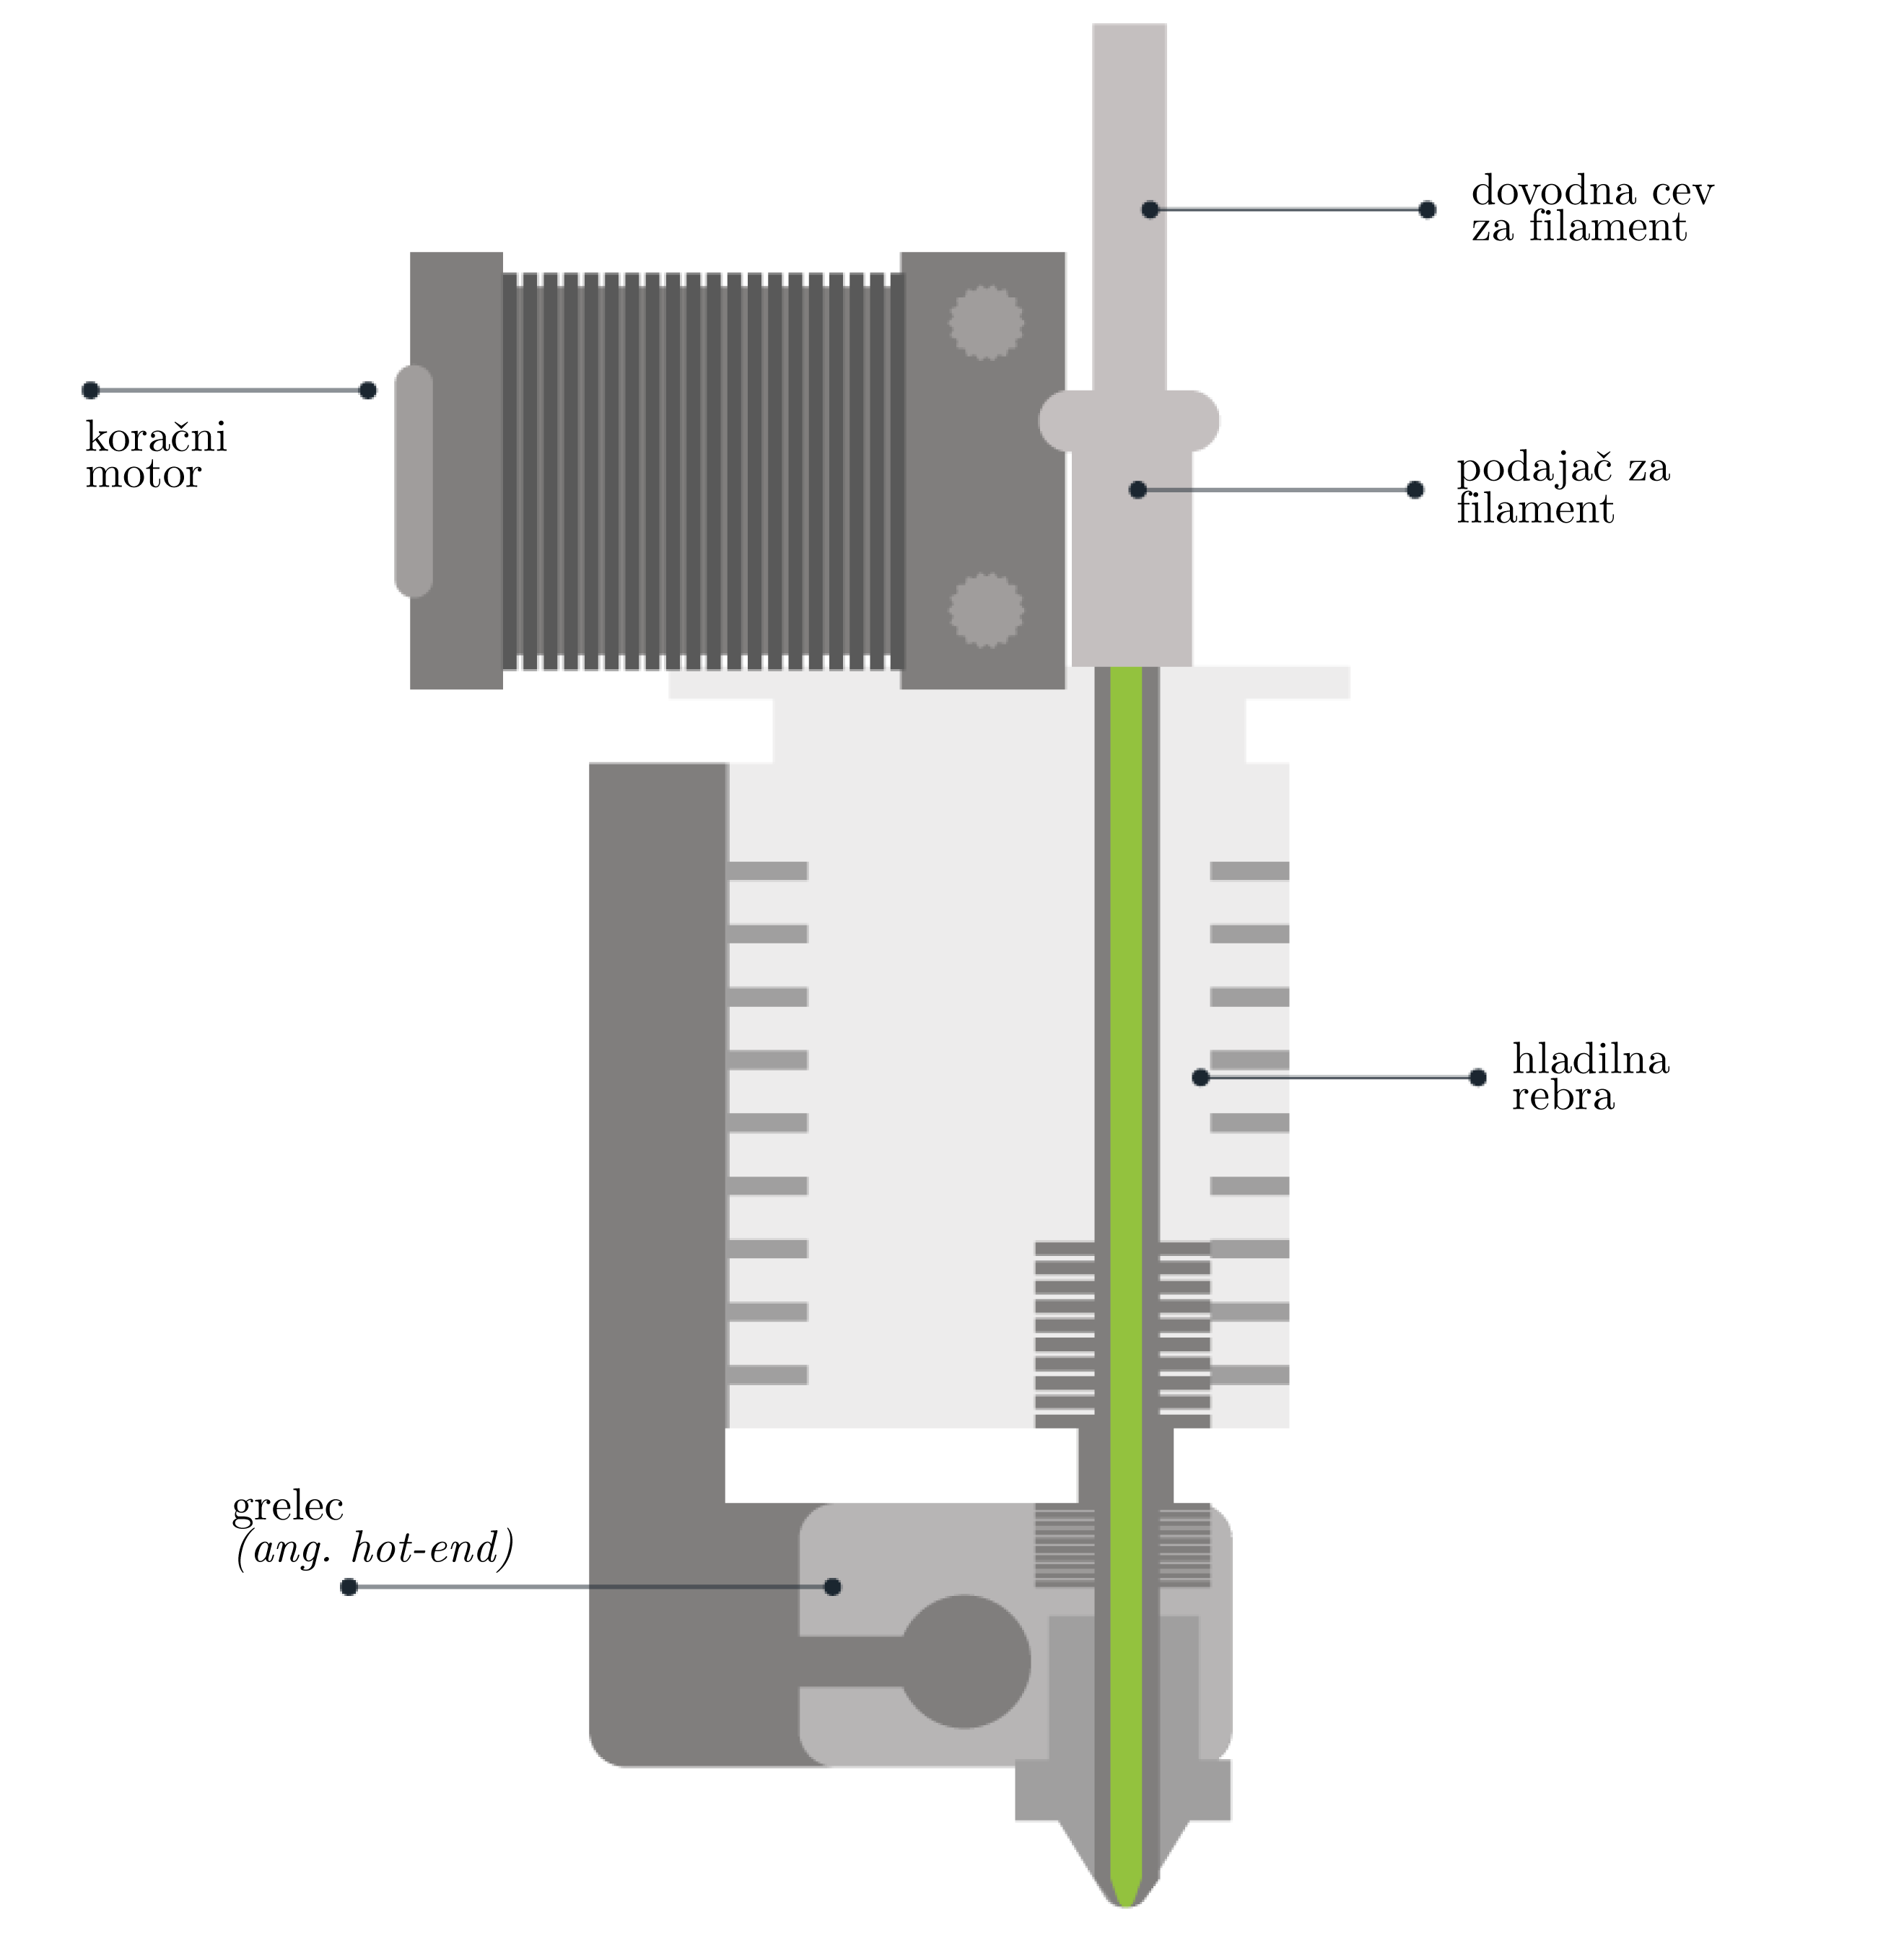
\includegraphics[scale=0.5]{Images/extruder.png}
  \caption{Glava FFF 3D tiskalnika in njeni sestavni deli \cite{leapfrog}}
\end{figure}
\noindent Za zagotavljanje najboljše kvalitete končnega izdelka, je pomemben konstanten in kontinuiran tok taljenega materiala. Za to skrbi koračni motor, ki filament potiska preko
podajača (zobnik). Ta mora imeti pravilno nastavljeno silo pritiska, da filament ne zdrsuje ali se lomi med podajanjem. \cite{fff_article}

\subsection{Karakterisike 3D tiskalnika}
\subsubsection{Parametri 3D tiska}
Pred začetkom 3D tiska je potrebna priprava datotke z zapisom informacij o izdelavi modela. Gre za G-kodo, ki vključuje podatke o premikanju motorjev, hitrosti podajanja filamenta, temperature plošče, temperature šobe in ogromno ostalih opcijskih parametrov.
Izbira pravilnih parametrov 3D tiska močno vpliva na uspešnost tiska in kvaliteto končnega izdelka. \\
Ločljivost končnega izdelka določimo z izbiro premera šobe in višino ekstrudirane plasti. Kljub temu, da lahko na dimenzijsko natančnost končnega izdelka vplivamo z veliko ostalimi parametri, sta debelina plasti in premer šobe ponavadi prva parametra, s katerima nadzorujemo
omenjeno lastnost. Z zmanjšanjem premera šobe in tanjšanjem debeline plasti, izboljšamo kvaliteto površin in detajlov. \cite{redwood20173d}
\\
Zelo pomembna je predvsem pravilna izbira temperature šobe in plošče. Ti temperaturi se močno razlikujeta od filamenta do filementa in sta ponavadi v območjih podani od proizvajalna filamenta. Končna določitev temperature je nato vedno rezultat 
izvedenih testnih izdelkov. Temperatura šobe je odvisna od temperature steklenja $T_g$ polimernega materiala, ki ga uporabljamo kot filament. Pri tej temperaturi pride do razpada šibkih Van der Waalsovih vezi, ki med seboj držijo povezane polimerne verige. Takrat filament začne izkazovati
manjšo viskoznost skupaj z ostalimi spremenjenimi visko-elastičnimi lastnostmi.

\subsubsection{Adhezija}
Med premikanjem plošče in glave je pomembno, da iztiskan material ostanee na prvotnem mestu, drugače dobimo zamike med plastmi. To dosežemo s pravilno adhezijo prve plasti na ploščo. Dobro adhezijo lahko dosežemo na več načinov, ki pa so vsi povezani z lastnostmi podlage.
Prvi parameter, ki vpliva na adhezijo prve plasti je temperatura plošče. S pravilno segreto podlago, zagotovimo dobro povezavo molekul, ki zagotovijo močno adhezijo. Pomagamo tudi s predpripravo plošče --- v ta namen obstajajo
različna sredstva in spreji, vendar zadostuje tudi lak za lase, kadar imamo stekleno ploščo, ali pa trdo ''UHU`` lepilo za druge podlage. \\
Tako kot adhezija prve plasti je pomembna tudi adhezija medsebojnih plasti. To dosežemo s pritiskom nove plasti na prejšnjo, pri čemer pomaga tudi delno ponovno taljenje predhodne plasti. Zaradi pritiska zgornje plasti se nalaganje dogaja v ovalni obliki, če bi opazovali presek. Stiki med dvema ovaloma predstavljajo mesta koncentracije napetosti, kjer najhitreje prihaja do loma. \cite{redwood20173d} Zaradi tega v smeri nalaganja plasti pričakujemo 
nizke mehanske lastnosti končnega izdelka.

\subsubsection{Podpore}
Čeprav je metoda \ac{FFF} 3D tiska zelo vsestranska ima svoje omejitve. Velik problem predstavljajo geometrije, kjer je naklon stene manjši od 45$^{\circ}$ glede na podlago. Nad to mejo se plasti ne sprimeta več dobro med seboj. Temu se lahko izognemo z uporabo podpornih stuktur. Te strukrue imajo majhno gostoto tiska in posebno geometrijo, ki porabi malo filamenta a zagotavlja veliko podporno površino in lahko odstranjevanje. 
S tem dodamo podlago, na katero se naslednja plast lahko odloži. Podporne strukture po končanem tisku nato odstranimo. Zaradi stika s podpornim materialom je kvaliteta površine slabša, zato
odstranjevanju podpornih struktur ponavadi sledi naknadna obelava izdelka.\cite{redwood20173d}

\subsubsection{Stopnja zapolnjenosti (ang. \emph{Infill})}
Z metodo \ac{FFF} ponavadi ne tiskamo popolnoma polnih izdelkov. Da se izognemo dolgim časom tiska in večji porabi materiala ponavadi izdelek zapolnimo le deloma. \cite{redwood20173d}
Med pripravo modela določimo debelino sten izdelka, ki so natisnjene polno in pa delež in geometrijo notranje zapolnitve. Geometrija je lahko heksagonalna, kvadratna, trikotna, itd. Z zmanjšanjem stopnje
zapolnitve močno skrajšamo čas tiska a hkrati tudi vplivamo na nižje mehanske lastnosti končnega izdelka.

\subsection{Dimenzijska natačnost}
3D natisnjeni izdelki so vedno izpostavljeni dimenzijskim napakam. Med procesom tiska pri posameznih nanesenih plasteh prihaja najprej do raztezanja in nato krčenja materiala zaradi temperaturnih
razlik. Pri tem se ustvarjajo notranje napetosti, ki vodijo do krčenja in krivljenja materiala. \cite{redwood20173d} Stopnja krčenja je neposredno odvisna od uporabljenega materiala. PLA filamenti so veliko bolj izpostavljeni krčenju kot PETG filamenti, slednji pa 
so veliko bolj dovzetni za krivljenje kot pa PLA filamenti. V kolikor je pomembno ujemanje med izdelki je potrebno prilagajanje dimenzij pred tiskom. 

\chapter{Zasnova in preračun metamateriala}
V tem poglavju je najprej predstavljena zasnovana \ac{OC} \ac{MM}. Sledi predstavitev izdelave programa za numerično simulacijo odziva \ac{MM} in izris disperzijskih krivulj po direktni
metodi.

\section{Zasnova oblike metamateriala}
Cilj zasnove je bila konstrukcija \ac{OC} \ac{MM}, ki omogoča 1D periodičnost. Zaradi lažjega prilagajanja tekom preizkusov je \ac{OC} zasnovana parametrično, kar omogoča hitre popravke
tako na nivoju CAD modela, kot tudi numeričnega izračuna. Po veliko iteracijah smo se odločili za obliko \ac{OC}, ki je prikazana na sliki (3.1). Zaradi parametričnosti lahko hitro spreminjamo 1. lastno frekvenco preko 
spreminjanja mase in togosti vzmeti resonatorja. Resonator se nahaja znotraj osnove strukture, saj tako ob nihanju strukture ne povzroča torzijskih obremenitev, prav tako pa se s tem
ognemo gibanju resonatorja v drugih smereh razen navzgor in navzdol.
\begin{figure}[H]
  \centering
  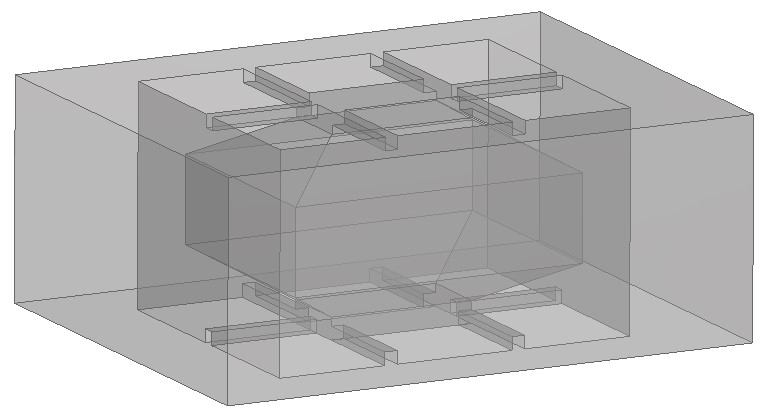
\includegraphics[scale=0.6]{Images/BaseCell_v4.JPG}
  \caption{Končni koncept \ac{OC} \ac{MM}}
\end{figure}
\noindent Pri zasnovi so bile že upoštevane tudi omejitve izdelave \ac{OC} s pomočjo FFF tehnike 3D tiska. Načrtovane vzmeti na omogočajo visoko uspešnost dobrega tiska
na dnu strukture in se zanašajo na pravilno izbrane parametre tiska pri zgornjih vzmeteh. Slednje namreč uporabljajo posebno tehniko 3D tiska imenovano ``mostiščenje'' (ang. bridging). Takrat tiskalnik nanaša material čez
večje vrzeli brez podpore. Na sliki (3.2) so prikazane končne mere \ac{OC}, ki smo jih prilagajali dokler lastna frekvenca strukture ni bila med 0 in 1000 Hz.
\\
Dvojne vzmeti na straneh so načrtovane zaradi preprečevanja nihanja notranje mase okoli z osi. Pri debelinah vzmeti smo omejeni z zmožnostjo izdelave s tehnologijo 3D tiska --- če bi
vzmeti naredili preozke ali pretanke bi prehitro prišlo do njihove porušitve.
\begin{figure}[H]
  \centering
  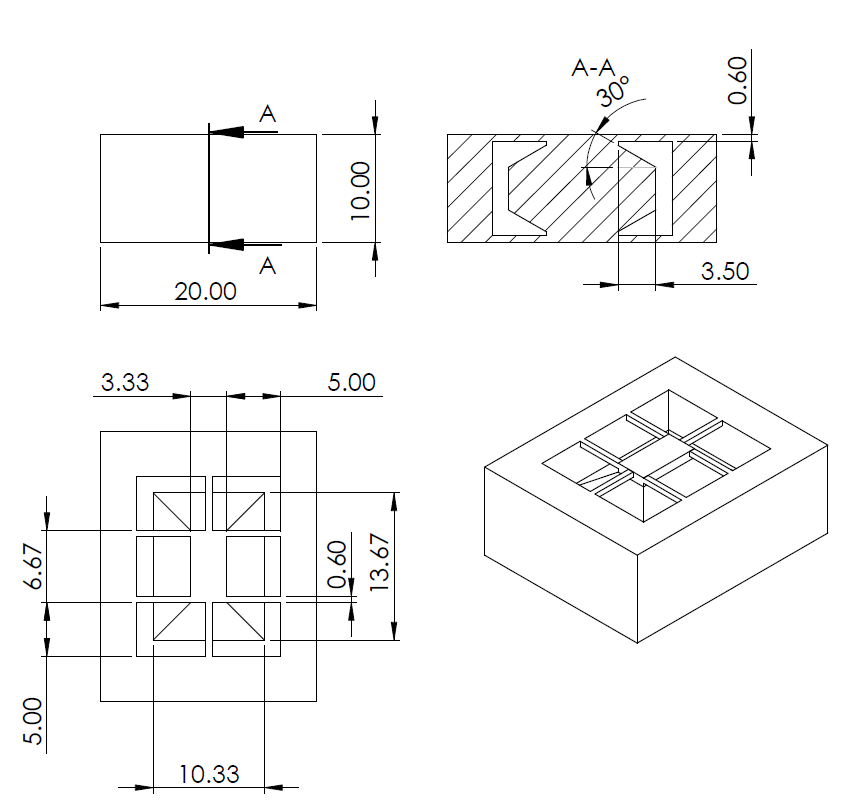
\includegraphics[scale=0.8]{Images/drawing.png}
  \caption{Dimenzije \ac{OC} \ac{MM}}
\end{figure}
Znotraj programskega paketa za CAD modeliranje Solidworks so za \ac{OC} parametrizirane naslednje veličine:
\begin{itemize}
  \item Širina, višina in dolžina \ac{OC};
  \item širina in debelina vzmeti.
\end{itemize}

\section{Izdelava numeričnega modela}
Dandanes imamo za numerične simulacije na voljo različne programske pakete, ki nam predvsem močno pomagajo pri analizi komopliciranih 2D ali 3D struktur. Ponavadi bi osnovne preračune naredili
v omenjenih paketih in bi potem s pridobljenimi podatki znotraj ločenega programa izračunali še disperzijske krivulje.
V našem primeru imamo relativno preprosto strukturo, zato je mogoče za vse narediti enoten program in se povsem ogniti uporabi programov drugih proizvajalcev.
\\
V tem poglavju bo obrazložen postopek izdelave numeričnega modela v programskem jeziku Python.

\subsection{Izračun lastnih frekvenc}
Program za analizo \ac{MM} je spisan v obliki razreda, ki mu podamo naslednje vhodne podatke:
\begin{itemize}
  \item Elastični modul;
  \item širina, višina in dolžina \ac{OC};
  \item gostota;
  \item nadomestna togost vzmeti;
  \item masa resonatorja;
  \item število končnih elementov.
\end{itemize}
Nadomestno togost vzmeti pridobimo s pomočjo strukturne analize \ac{OC} v programskem paketu Ansys \cite{ansys}, maso resonatroja pa iz CAD modela iz programskega paketa Solidworks \cite{solidworks}. Program v naslednjih korakih tvori globalno masno in togostno matriko
sistema, pri čemer upošteva spremenljiv prerez, ki vpliva na površino prereza in vztrajnostni moment prereza. Nato globalni matriki recudira v reducirano globalno masno in reducirano globalno
togostno matriko. Vse te matrike so funkcije vektorja širjenja valovanja $\mu$. Ko rešimo \ac{EVP} dobimo seznam lastnih frekvenc in lastnih oblik, katerega dolžina je enaka številu končnih elementov. Seznam prav tako pripada točno določenemu vektorju širjenja valovanja.

\subsection{Izračun disperzijskih krivulj}
V naslednjem koraku po inverznem pristopu izračunamo disperzijske krivulje za pripadajoči \ac{MM}. Program to naredi tako, da za končno število vektorjev širjenja valovanja $\mu$ s postopkom iz poglavja 3.2.1 izračuna
lastne frekvence in jih nariše na graf $\omega(\mu)$. Zaradi preglednosti v programu lahko izberemo koliko lastnih frekvenc prikažemo na grafu in omejimo njegovo območje frekvenc, da lažje določimo \ac{PZF}.
Program nato izračuna razliko med najmanjšo vrednostjo druge lastne frekvence in največjo vrednostjo prve lastne frekvence in izriše območje \ac{PZF}. Disperzijka krivulja je razvidna iz slike (3.3).
\begin{figure}[H]
  \centering
  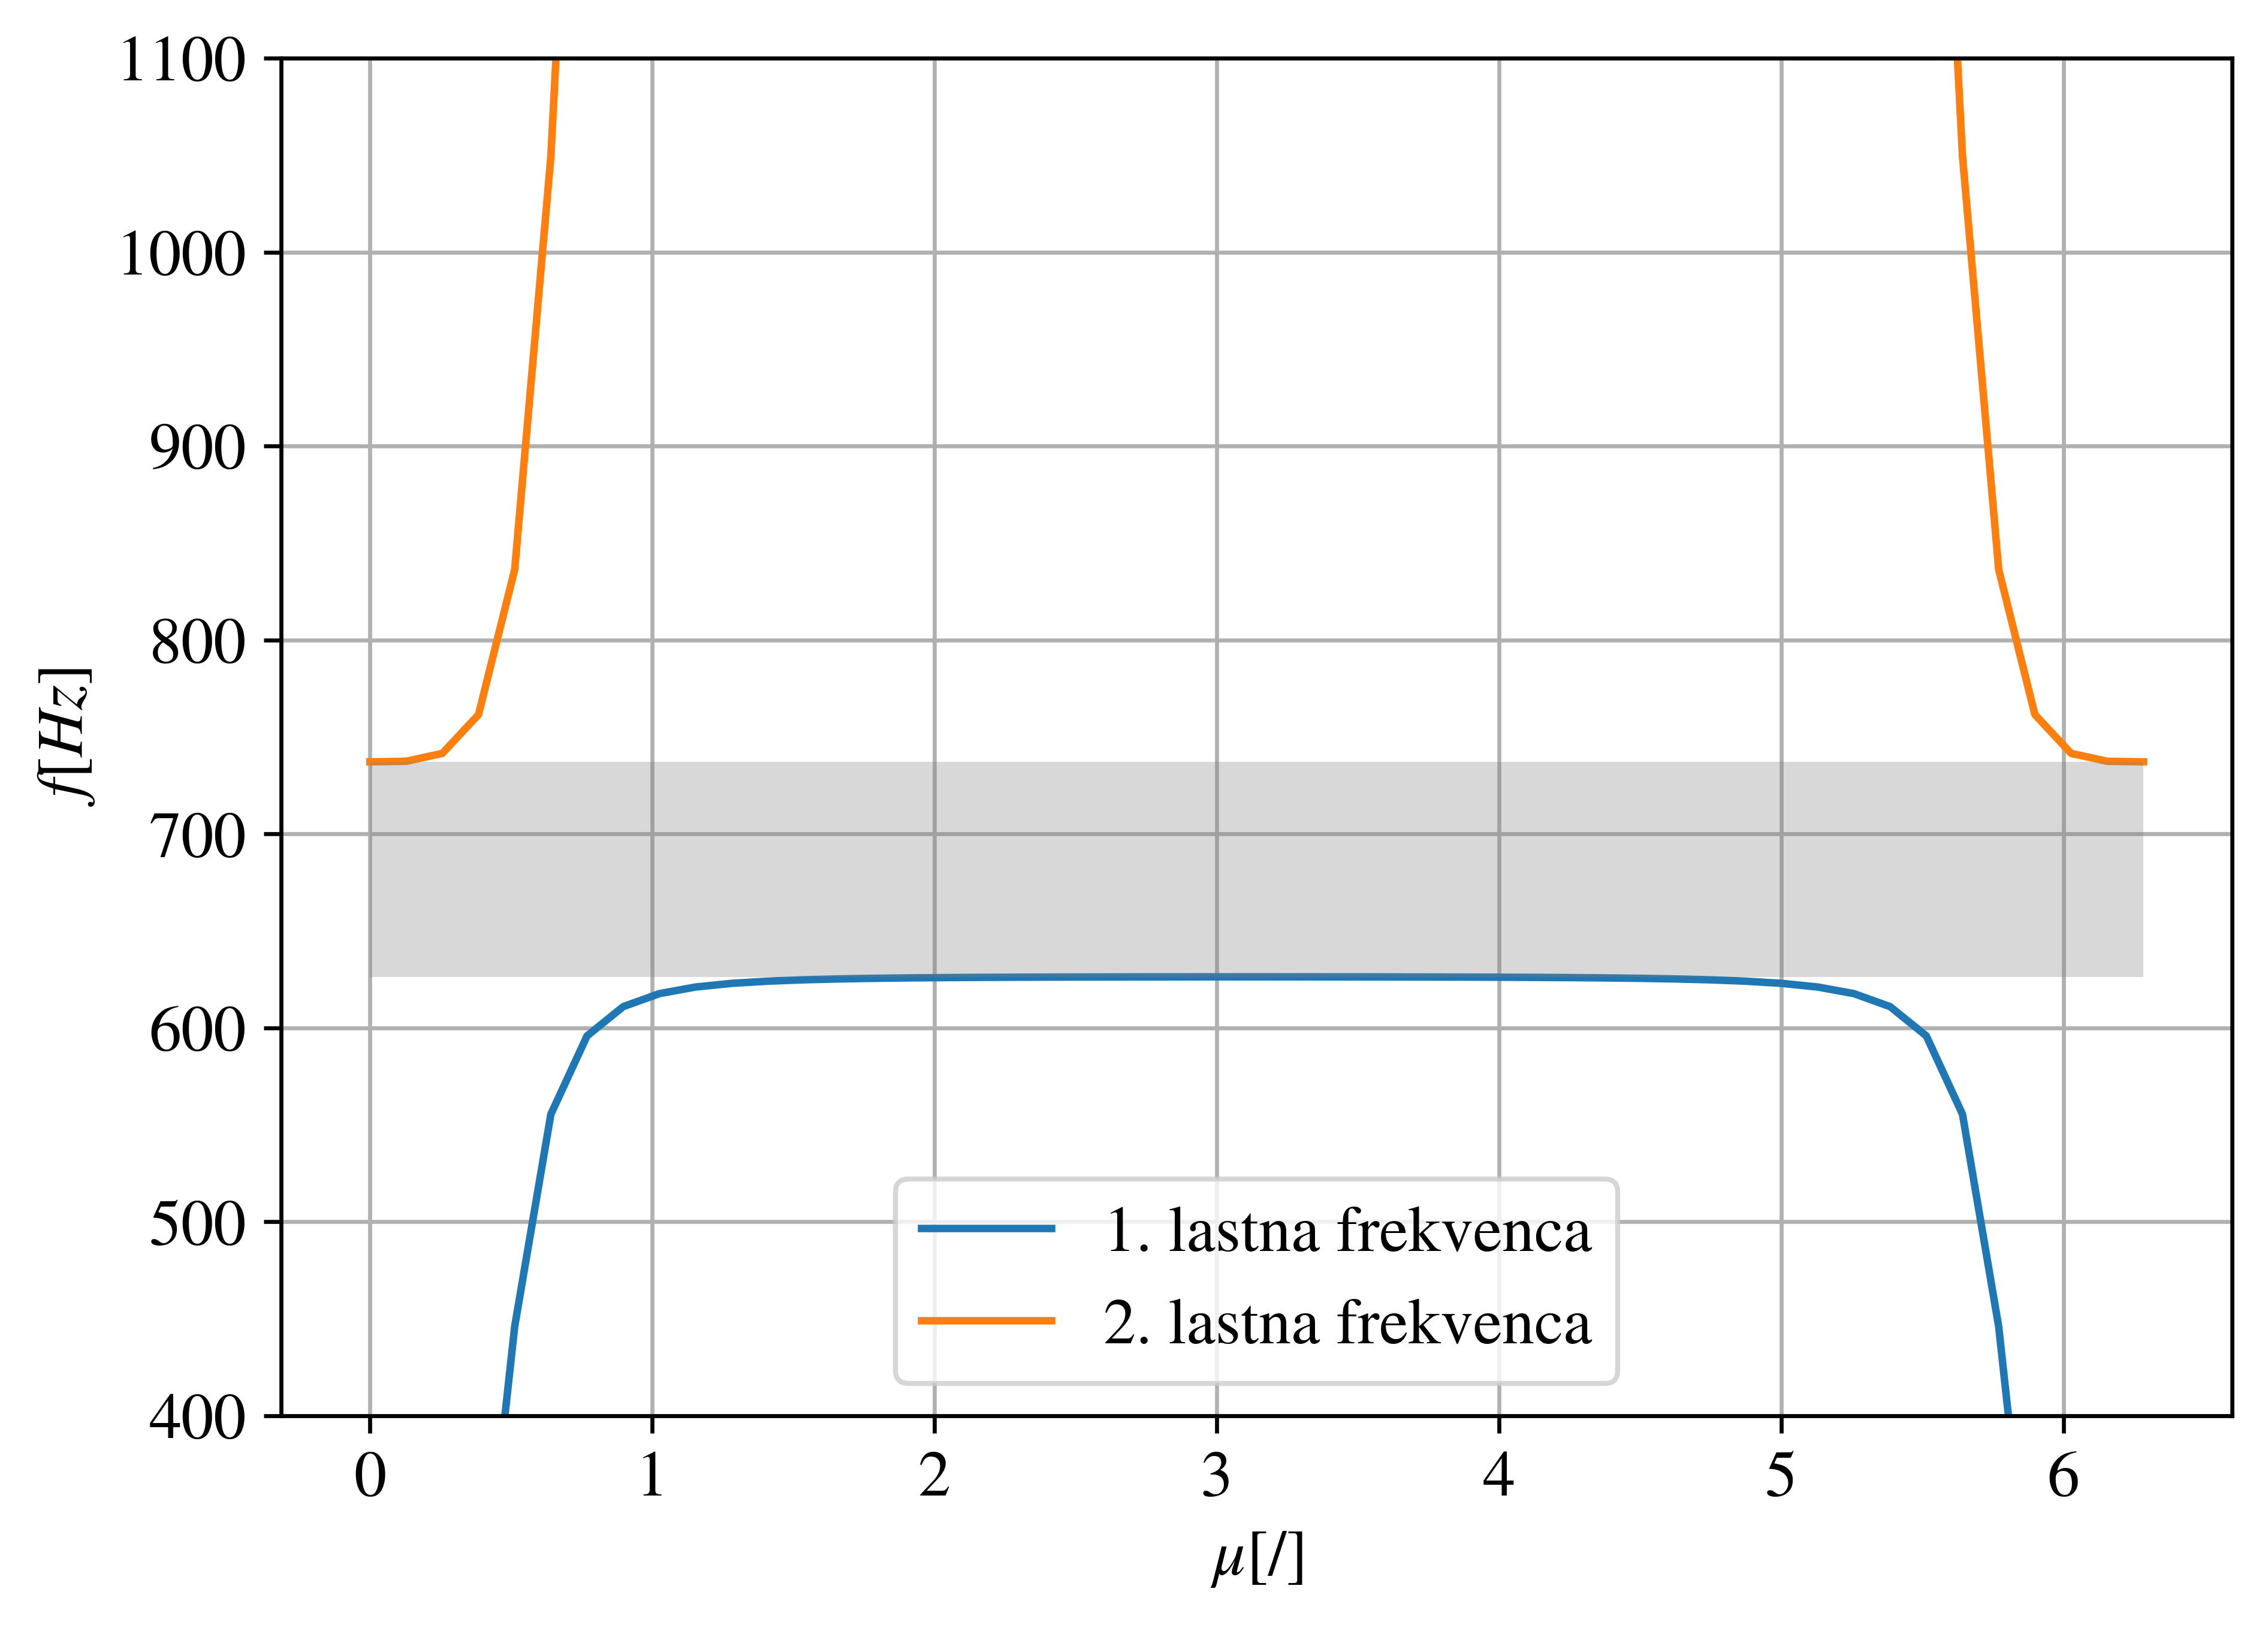
\includegraphics[scale=0.6]{Images/dispersion.png}
  \caption{Disperzijske krivulje za \ac{MM}}
\end{figure}
Iz diagrama je razvidno, da naj bi \ac{PZF} bil med 800 in 950 Hz. Po analizah v programskem paketu Ansys \cite{ansys}, se v tem območju nahaja tudi prva lastna frekvenca
\ac{OC}, kjer resonator intenzivno niha navzgor in navzdol.

\subsection{Simulacija odziva \ac{MM}}
Da si je lažje predstavljati različno obnašanje strukture pri različnih vektorjih širjenja valovanja, program vsebuje tudi tudi metodo za vizualizacijo relativnega gibanja osnovne strukture
in resonatorja. Oblike lahko izrišemo s pomočjo vektorja lastnih oblik, ki ga dobimo poleg vektorja lastnih frekvenc kot rezultat rešive \ac{EVP}. Preden pa obliko lahko izrišemo, moramo dodati manjkajoča
vozlišča, saj smo matriko pred tem reducirali. Prav tako v tej stopnji v simulacijo dodamo več osnovnih celic, da dobimo obliko nosilca. V ta namen uporabimo Bloch-Floquetov teorem, ki povezuje skrajne točke \ac{OC}.
Vektor pomikov je kompleksen --- realne komponente predstavljajo razmerje pomikov, imaginarne komponente pa fazni zamik, ki ga moramo prav tako upoštevati. Na slikah (3.4) - (3.10) so predstavljene zamrznjene slike iz simulacije pri 
različnih vektorjih širjenja valovanja. 
\begin{figure}[H]
  \centering
  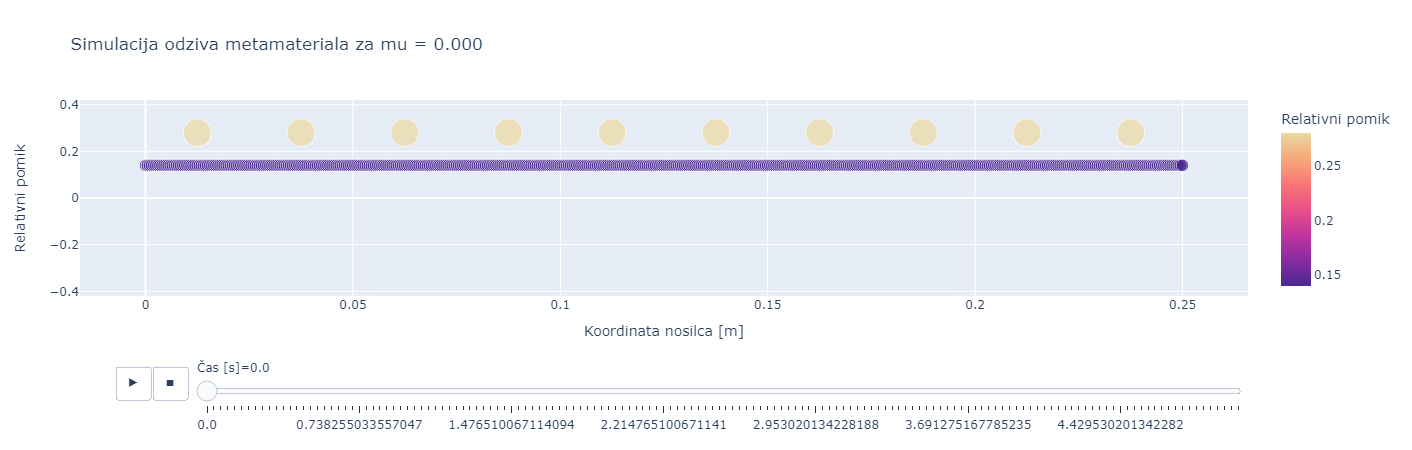
\includegraphics[trim={0 4cm 0 3.5cm},clip, scale=0.3]{Images/mu0.png}
  \caption{Simulacija za $\mu = 0$}
\end{figure}
\begin{figure}[H]
  \centering
  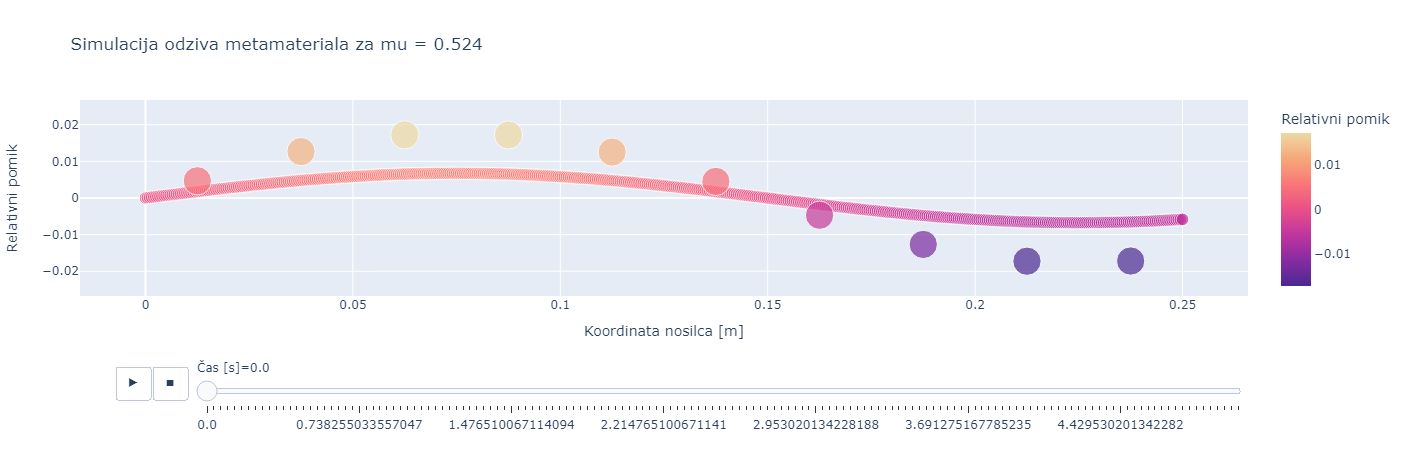
\includegraphics[trim={0 4cm 0 3.5cm},clip, scale=0.3]{Images/mupi_6.png}
  \caption{Simulacija za $\mu = \frac{\pi}{6}$}
\end{figure}
\begin{figure}[H]
  \centering
  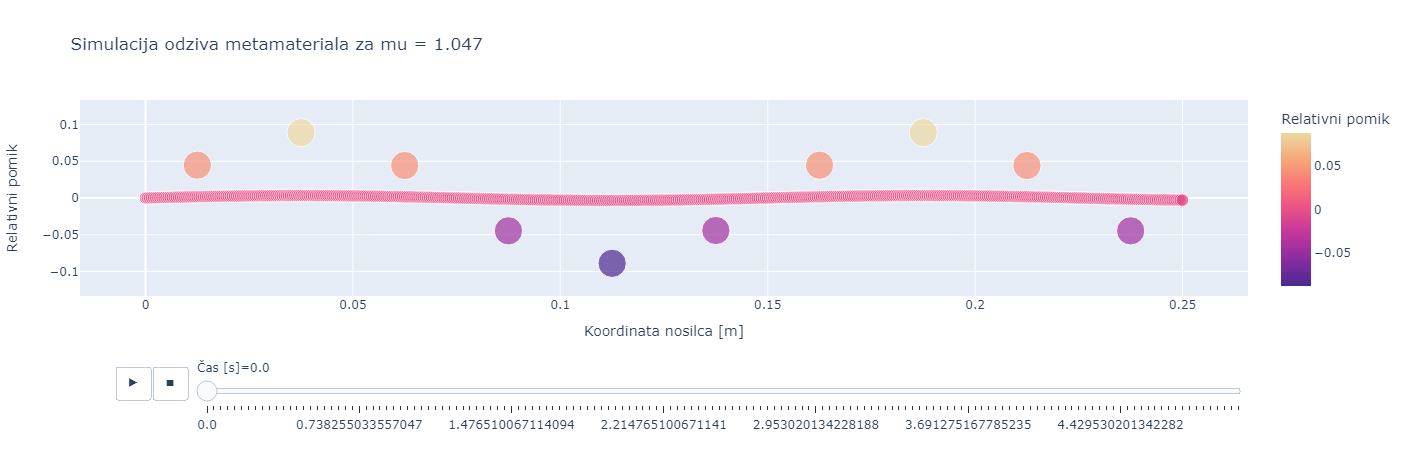
\includegraphics[trim={0 4cm 0 3.5cm},clip, scale=0.3]{Images/mupi_3.png}
  \caption{Simulacija za $\mu = \frac{\pi}{3}$}
\end{figure}
\begin{figure}[H]
  \centering
  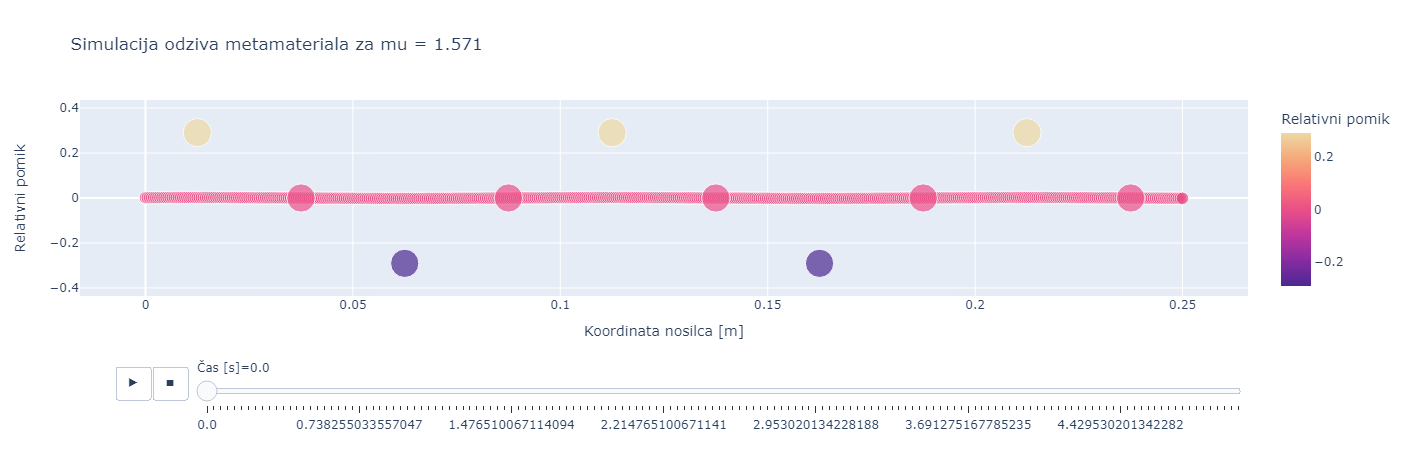
\includegraphics[trim={0 4cm 0 3.5cm},clip, scale=0.3]{Images/mupi_2.png}
  \caption{Simulacija za $\mu = \frac{\pi}{2}$}
\end{figure}
\begin{figure}[H]
  \centering
  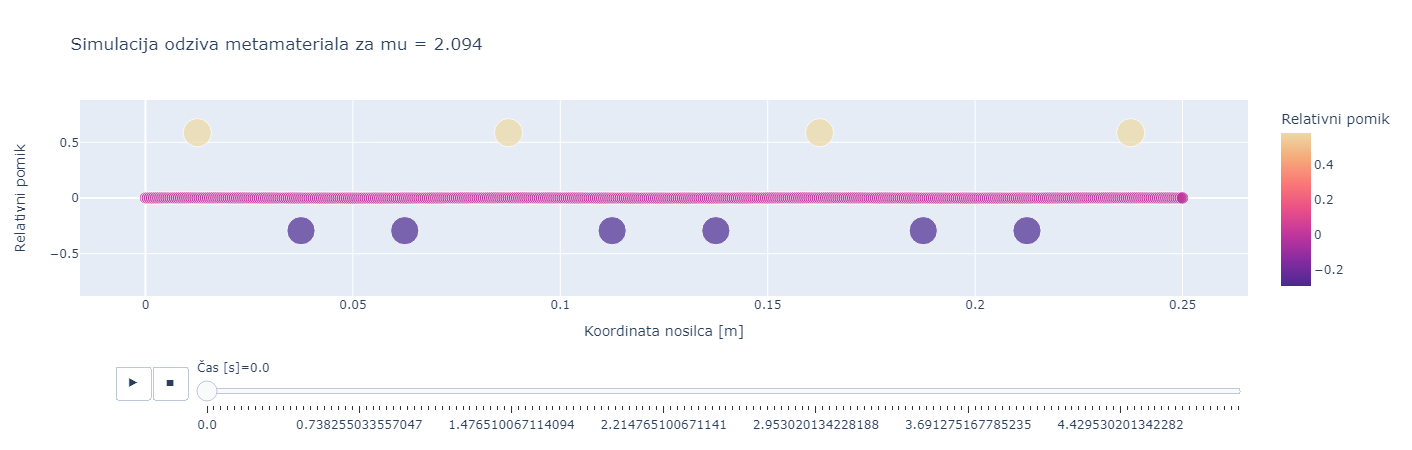
\includegraphics[trim={0 4cm 0 3.5cm},clip, scale=0.3]{Images/mu2pi_3.png}
  \caption{Simulacija za $\mu = \frac{2\pi}{3}$}
\end{figure}
\begin{figure}[H]
  \centering
  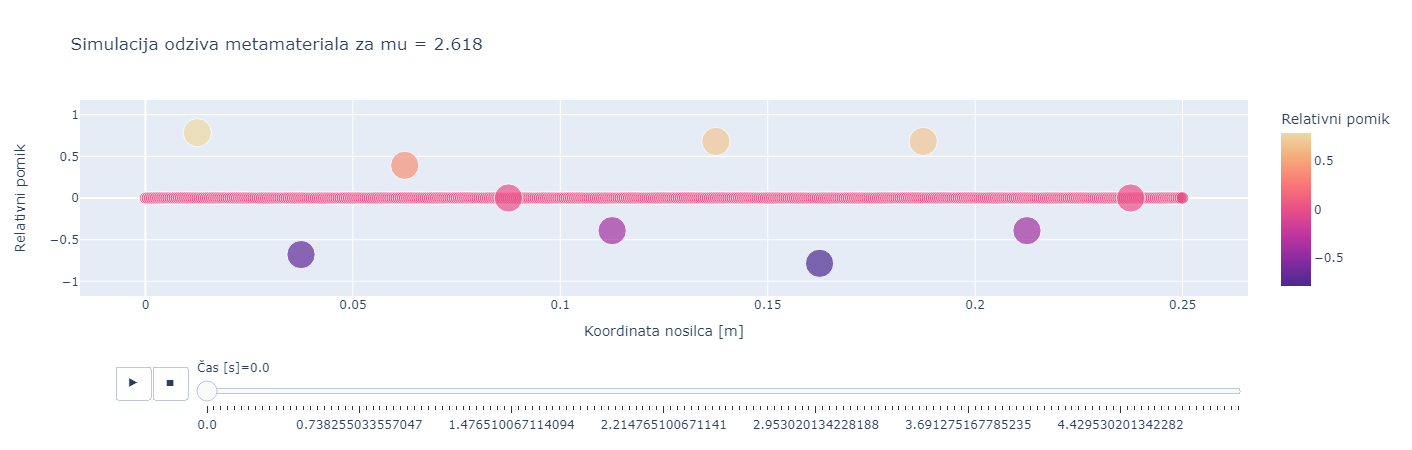
\includegraphics[trim={0 4cm 0 3.5cm},clip, scale=0.3]{Images/mu5pi_6.png}
  \caption{Simulacija za $\mu = \frac{5\pi}{6}$}
\end{figure}
\begin{figure}[H]
  \centering
  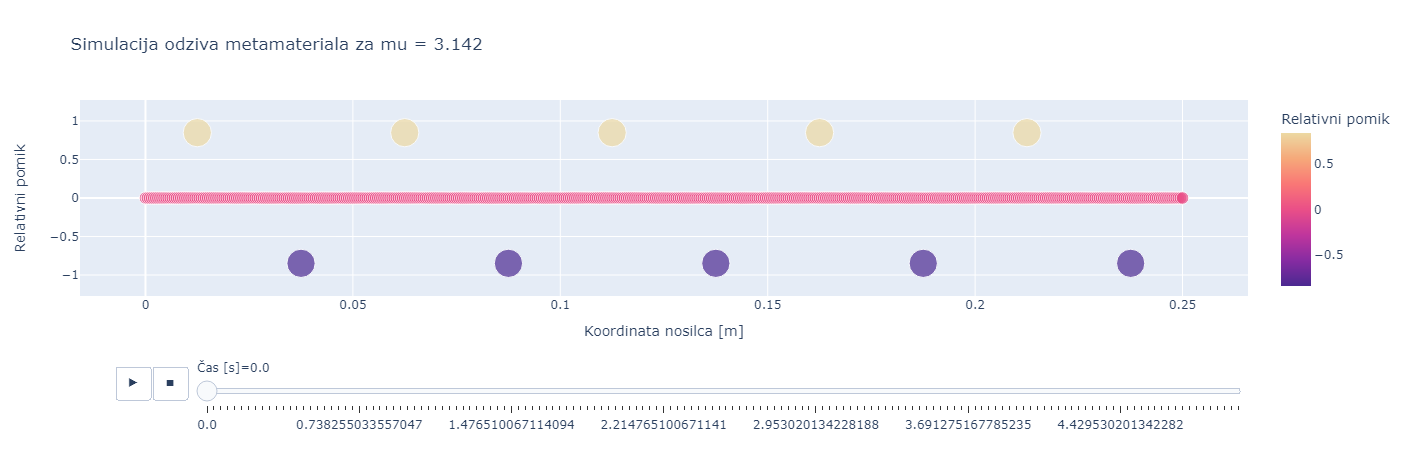
\includegraphics[trim={0 4cm 0 3.5cm},clip, scale=0.3]{Images/mupi.png}
  \caption{Simulacija za $\mu = \pi$}
\end{figure}
\noindent Na slikah manjša pike predstavljajo vozlišča končnih elementov osnovne strukture, večje pike pa resonatorje.



\chapter{Eksperimentalni del}
V tem poglavju bomo predstavili postopek določanja materialnih lastnosti filamenta in 3D tiska \ac{MM}. Temu bo sledila predstavitev eksperimenta in primerjava rezultatov z numeričnimi 
napovedmi iz poglavja 3.

\section{Proces 3D tiska}
Po končani konstrukciji \ac{OC} \ac{MM}, smo iz programskega paketa Solidworks \cite{solidworks} v formatu STL. STL zapis model razdeli na trikotnike, s katerimi popiše površine izdelka. Naslednji korak je bil priprava G-kode za 3D tiskalnik. V ta namen obstaja več namenskih programskih paketov, ki model za dane parametri razreže na plasti (ang. \emph{slicing}) in tvori
G-kodo. Mi smo uporbili prosto dostopni program UltiMaker Cura \cite{cura}. \\
Za izdelavo \ac{MM} smo uporabili PETG filament. V primerjavi z bolj razširjeno uporaljenim PLA filamentom ima PETG boljšo fleksibilnost, kar potrebujemo za vzmetni del \ac{OC}.

\begin{table}[H]
  \caption{Osnovni parametri za tisk}
  \centering
  \begin{tabular}{ | l | c | r | }
    \hline
    Temperatura šobe & 240 $^{\circ}$ \\ \hline
    Temperatura podloge & 82 $^{\circ}$ \\ \hline
    Delež zapolnitve & 100 \% \\ \hline
    Hitrost tiska & 50 mm s$^{-1}$ \\ \hline
    Debelina plasti & 0.15 mm \\ \hline
    Hitrost mostiščenja & 10 mm s$^{-1}$ \\
    \hline  
  \end{tabular}
\end{table}

\noindent Posebej pozorni smo bili na vzmeti \ac{OC} \ac{MM}, saj so ključnega pomena za pravilno območje \ac{PZF}. Vzmeti so izjemno majhnih dimenzij (0.6 mm x 0.6 mm) in se nahajajo na zgornjem
in spodnjem delu \ac{OC}. Na spodnjem delu vzmeti ležijo neposredno na plošči, kar ne predstavlja nobenega problema, medtem ko na zgornjem delu nimajo nobenega podpornega materiala. Praviloma bi v takem
primeru uporabili podporne strukture, vendar je razdalja majhna, prav tako pa bi bilo po tisku podpore nemogoče odstraniti zaradi nedostopnosti. V takem primeru se poslužimo posebne tehnike ''mostiščenja`` (ang. \emph{bridging}), kjer lahko
material nanašamo med dvema stenama brez podpor. Da je to izvedljivo je potrebno na tem mestu prilagoditi parametre tiskanja --- močno upočasniti hitrost tiska in povečati hlajenje na maksimalno raven, da se material v trenutku strdi. S tem močno izboljšamo
uspešnost tiska brez podpor.

\begin{figure}[H]
  \centering
  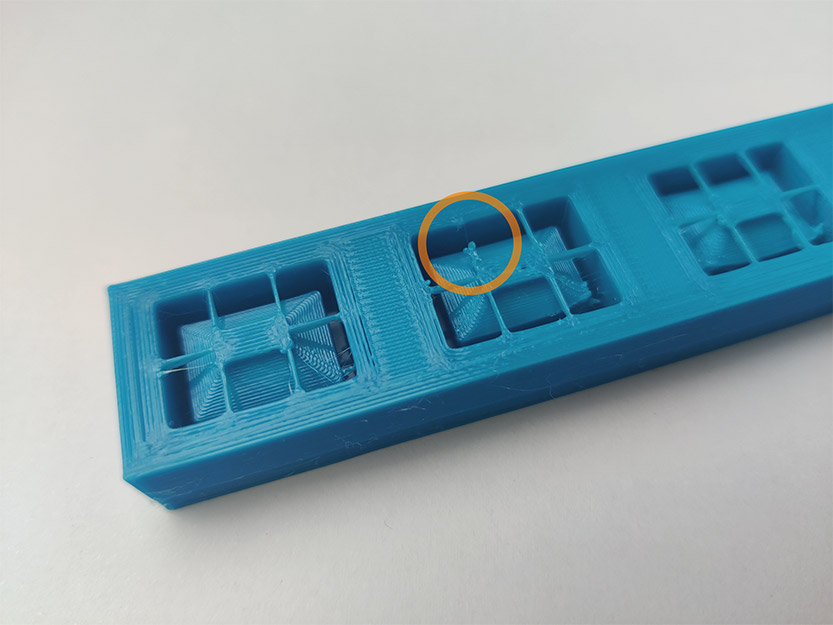
\includegraphics[scale=0.4]{Images/mostiscenje_small.jpg}
  \caption{Primer slabega mostiščenja}
\end{figure}
\noindent Tisk ene enote nosilca, ki je zaradi velikosti plošče tiskalnika omejena na 25 cm, je trajala 7 ur.

\section{Meritve}


\printbibliography[heading=bibnumbered]
%\addcontentsline{toc}{chapter}{Literatura}
\end{document}